\documentclass[notoc]{tufte-book}
\usepackage{fontawesome5}
\hypersetup{colorlinks}% uncomment this line if you prefer colored hyperlinks (e.g., for onscreen viewing)

%%
% Book metadata





\title{{Applied Microeconometrics}}

\author[Aakash Ghosh]{Aakash Ghosh (19MS129)}







%%
% If they're installed, use Bergamo and Chantilly from www.fontsite.com.
% They're clones of Bembo and Gill Sans, respectively.
%\IfFileExists{bergamo.sty}{\usepackage[osf]{bergamo}}{}% Bembo
%\IfFileExists{chantill.sty}{\usepackage{chantill}}{}% Gill Sans

%\usepackage{microtype}

%%
% Just some sample text
\usepackage{lipsum}

%%
% For nicely typeset tabular material
\usepackage{booktabs}

%%
% For graphics / images
\usepackage{graphicx}
\setkeys{Gin}{width=\linewidth,totalheight=\textheight,keepaspectratio}
\graphicspath{{graphics/}}

% The fancyvrb package lets us customize the formatting of verbatim
% environments.  We use a slightly smaller font.
\usepackage{fancyvrb}
\fvset{fontsize=\normalsize}

%%
% Prints argument within hanging parentheses (i.e., parentheses that take
% up no horizontal space).  Useful in tabular environments.
\newcommand{\hangp}[1]{\makebox[0pt][r]{(}#1\makebox[0pt][l]{)}}

%%
% Prints an asterisk that takes up no horizontal space.
% Useful in tabular environments.
\newcommand{\hangstar}{\makebox[0pt][l]{*}}

%%
% Prints a trailing space in a smart way.
\usepackage{xspace}

%%
% Some shortcuts for Tufte's book titles.  The lowercase commands will
% produce the initials of the book title in italics.  The all-caps commands
% will print out the full title of the book in italics.
\newcommand{\vdqi}{\textit{VDQI}\xspace}
\newcommand{\ei}{\textit{EI}\xspace}
\newcommand{\ve}{\textit{VE}\xspace}
\newcommand{\be}{\textit{BE}\xspace}
\newcommand{\VDQI}{\textit{The Visual Display of Quantitative Information}\xspace}
\newcommand{\EI}{\textit{Envisioning Information}\xspace}
\newcommand{\VE}{\textit{Visual Explanations}\xspace}
\newcommand{\BE}{\textit{Beautiful Evidence}\xspace}

\newcommand{\TL}{Tufte-\LaTeX\xspace}

% Prints the month name (e.g., January) and the year (e.g., 2008)
\newcommand{\monthyear}{%
	\ifcase\month\or January\or February\or March\or April\or May\or June\or
	July\or August\or September\or October\or November\or
	December\fi\space\number\year
}


% Prints an epigraph and speaker in sans serif, all-caps type.
\newcommand{\openepigraph}[2]{%
	%\sffamily\fontsize{14}{16}\selectfont
	\begin{fullwidth}
	\sffamily\large
	\begin{doublespace}
	\noindent\allcaps{#1}\\% epigraph
	\noindent\allcaps{#2}% author
	\end{doublespace}
	\end{fullwidth}
}

% Inserts a blank page
\newcommand{\blankpage}{\newpage\hbox{}\thispagestyle{empty}\newpage}

\usepackage{units}

% Typesets the font size, leading, and measure in the form of 10/12x26 pc.
\newcommand{\measure}[3]{#1/#2$\times$\unit[#3]{pc}}

% Macros for typesetting the documentation
\newcommand{\hlred}[1]{\textcolor{Maroon}{#1}}% prints in red
\newcommand{\hangleft}[1]{\makebox[0pt][r]{#1}}
\newcommand{\hairsp}{\hspace{1pt}}% hair space
\newcommand{\hquad}{\hskip0.5em\relax}% half quad space
\newcommand{\TODO}{\textcolor{red}{\bf TODO!}\xspace}
\newcommand{\na}{\quad--}% used in tables for N/A cells
\providecommand{\XeLaTeX}{X\lower.5ex\hbox{\kern-0.15em\reflectbox{E}}\kern-0.1em\LaTeX}
\newcommand{\tXeLaTeX}{\XeLaTeX\index{XeLaTeX@\protect\XeLaTeX}}
% \index{\texttt{\textbackslash xyz}@\hangleft{\texttt{\textbackslash}}\texttt{xyz}}
\newcommand{\tuftebs}{\symbol{'134}}% a backslash in tt type in OT1/T1
\newcommand{\doccmdnoindex}[2][]{\texttt{\tuftebs#2}}% command name -- adds backslash automatically (and doesn't add cmd to the index)
\newcommand{\doccmddef}[2][]{%
	\hlred{\texttt{\tuftebs#2}}\label{cmd:#2}%
	\ifthenelse{\isempty{#1}}%
		{% add the command to the index
			\index{#2 command@\protect\hangleft{\texttt{\tuftebs}}\texttt{#2}}% command name
		}%
		{% add the command and package to the index
			\index{#2 command@\protect\hangleft{\texttt{\tuftebs}}\texttt{#2} (\texttt{#1} package)}% command name
			\index{#1 package@\texttt{#1} package}\index{packages!#1@\texttt{#1}}% package name
		}%
}% command name -- adds backslash automatically
\newcommand{\doccmd}[2][]{%
	\texttt{\tuftebs#2}%
	\ifthenelse{\isempty{#1}}%
		{% add the command to the index
			\index{#2 command@\protect\hangleft{\texttt{\tuftebs}}\texttt{#2}}% command name
		}%
		{% add the command and package to the index
			\index{#2 command@\protect\hangleft{\texttt{\tuftebs}}\texttt{#2} (\texttt{#1} package)}% command name
			\index{#1 package@\texttt{#1} package}\index{packages!#1@\texttt{#1}}% package name
		}%
}% command name -- adds backslash automatically
\newcommand{\docopt}[1]{\ensuremath{\langle}\textrm{\textit{#1}}\ensuremath{\rangle}}% optional command argument
\newcommand{\docarg}[1]{\textrm{\textit{#1}}}% (required) command argument
\newenvironment{docspec}{\begin{quotation}\ttfamily\parskip0pt\parindent0pt\ignorespaces}{\end{quotation}}% command specification environment
\newcommand{\docenv}[1]{\texttt{#1}\index{#1 environment@\texttt{#1} environment}\index{environments!#1@\texttt{#1}}}% environment name
\newcommand{\docenvdef}[1]{\hlred{\texttt{#1}}\label{env:#1}\index{#1 environment@\texttt{#1} environment}\index{environments!#1@\texttt{#1}}}% environment name
\newcommand{\docpkg}[1]{\texttt{#1}\index{#1 package@\texttt{#1} package}\index{packages!#1@\texttt{#1}}}% package name
\newcommand{\doccls}[1]{\texttt{#1}}% document class name
\newcommand{\docclsopt}[1]{\texttt{#1}\index{#1 class option@\texttt{#1} class option}\index{class options!#1@\texttt{#1}}}% document class option name
\newcommand{\docclsoptdef}[1]{\hlred{\texttt{#1}}\label{clsopt:#1}\index{#1 class option@\texttt{#1} class option}\index{class options!#1@\texttt{#1}}}% document class option name defined
\newcommand{\docmsg}[2]{\bigskip\begin{fullwidth}\noindent\ttfamily#1\end{fullwidth}\medskip\par\noindent#2}
\newcommand{\docfilehook}[2]{\texttt{#1}\index{file hooks!#2}\index{#1@\texttt{#1}}}
\newcommand{\doccounter}[1]{\texttt{#1}\index{#1 counter@\texttt{#1} counter}}

% Generates the index
\usepackage{makeidx}
\makeindex


\usepackage{amsmath}


\newtheorem{defn}{Definition}
\newtheorem{theorem}{Theorem}
\newtheorem{corollary}{Corollary}[theorem]
\newtheorem{lemma}[theorem]{Lemma}


\definecolor{c1}{HTML}{000000}
\definecolor{c2}{HTML}{1E5128}
\definecolor{c5}{HTML}{4E9F3D}


\definecolor{c3}{HTML}{4E9F3D}
\definecolor{c4}{HTML}{F2FFE9}

% chapter format
\titleformat{\chapter}%
  {\huge\rmfamily\itshape\color{c1}}% format applied to label+text
  {\llap{\colorbox{c1}{\parbox{1.5cm}{\hfill\itshape\huge\color{white}\thechapter}}}}% label
  {2pt}% horizontal separation between label and title body
  {}% before the title body
  []% after the title body

% section format
\titleformat{\section}%
  {\normalfont\Large\itshape\color{c2}}% format applied to label+text
  {\llap{\colorbox{c2}{\parbox{1.5cm}{\hfill\color{white}\thesection}}}}% label
  {1em}% horizontal separation between label and title body
  {}% before the title body
  []% after the title body

% subsection format
\titleformat{\subsection}%
  {\normalfont\large\itshape\color{c5}}% format applied to label+text
  {\llap{\colorbox{c5}{\parbox{1.5cm}{\hfill\color{white}\thesubsection}}}}% label
  {1em}% horizontal separation between label and title body
  {}% before the title body
  []% after the title body

  \setcounter{secnumdepth}{2}


\usepackage {tfrupee}

\let\orupee\rupee
\def\rupee{\ifmmode\text{\orupee}\else\orupee\fi}

\usepackage{tcolorbox}
\usepackage{amsthm}
\usepackage{listings}
\usepackage{color}
\usepackage{tikz,lipsum,lmodern}
\definecolor{dkgreen}{rgb}{0,0.6,0}
\definecolor{gray}{rgb}{0.5,0.5,0.5}
\definecolor{mauve}{rgb}{0.58,0,0.82}


\usepackage{physics}
\usepackage{amsmath}
\usepackage{tikz}
\usepackage{mathdots}
\usepackage{yhmath}
\usepackage{cancel}
\usepackage{color}
\usepackage{array}
\usepackage{multirow}
\usepackage{amssymb}
\usepackage{gensymb}
\usepackage{tabularx}
\usepackage{extarrows}
\usepackage{booktabs}
\usetikzlibrary{fadings}
\usetikzlibrary{patterns}
\usetikzlibrary{shadows.blur}
\usetikzlibrary{shapes}

\setcounter{tocdepth}{2}


\usepackage{hyperref}
\hypersetup{
    colorlinks=true,
    linkcolor=c2
    }

\usepackage{listings}
\usepackage{color}

\definecolor{dkgreen}{rgb}{0,0.6,0}
\definecolor{gray}{rgb}{0.5,0.5,0.5}
\definecolor{mauve}{rgb}{0.58,0,0.82}

\lstset{frame=tb,
  language=R,
  aboveskip=3mm,
  belowskip=3mm,
  showstringspaces=false,
  columns=flexible,
  basicstyle={\small\ttfamily},
  numbers=none,
  numberstyle=\tiny\color{gray},
  keywordstyle=\color[HTML]{172774},
  commentstyle=\color[HTML]{EEEEEE},
  stringstyle=\color[HTML]{E94560},
  breaklines=true,
  breakatwhitespace=true,
  tabsize=3
}
\usepackage{ stmaryrd }


\makeatletter
% Paragraph indentation and separation for normal text
\renewcommand{\@tufte@reset@par}{%
  \setlength{\RaggedRightParindent}{0.0pc}%
  \setlength{\JustifyingParindent}{0.0pc}%
  \setlength{\parindent}{0pc}%
  \setlength{\parskip}{0pt}%
}
\@tufte@reset@par
\makeatother

\tcbuselibrary{breakable}

\begin{document}



\maketitle




% r.5 contents
\tableofcontents


\lstset{language=R}
\chapter{Basic Modelling and Linear Regression using OLS}
\section{Introduction}
    We shall mainly deal with micro data\sidenote{Macro data can be in a sense considered to be aggregate of micro data} on economic variables. The main objectives are:
    \begin{enumerate}
        \item \textbf{Causal analysis:} We try to differentiate between correlation and causation. For example: 2 rocks falling from a hill is a correlation as one doesn't cause the other. If a rock hits other, and they move, then it's causation: one causes the other.
        \item \textbf{Economic modelling:} We shall see economic models are good for causal analysis but not so good for forecasts\sidenote{On the other hand Machine learning models are very good in forecasts.}
    \end{enumerate}
\section{Linear models}
Consider the equation:
\begin{align}
  y=\alpha+\beta x+\epsilon  
\end{align}

Here, $y$ is the dependent variable or outcome and $x$ is the independent variable or the variable which causes change in $y$. It is also called the regressor or observed factor. $\epsilon$ is random error due to unobserved factors. Without $\epsilon$ the model becomes deterministic; with $\epsilon$ it is stochastic. We assume:
$$E[\epsilon|x]=0$$
From this assumption we have - 
$E[\epsilon]=0$ and  $Cov(x,\epsilon)=0$.{ This implies $x$ and $\epsilon$ are uncorrelated and that the errors are random}. $\alpha,  \beta$ are the parameters of the model. We define $\alpha=E[y|x=0]$ and $\beta=E\left[\frac{\partial y}{\partial x}\right]$. $\beta$ is also defined as the marginal effect of $x$ on $y$.



\subsection{Normal equations}
Note that From (1) we have $\epsilon=y-\beta x-\alpha $. Applying $E[\epsilon]=0$ and  $Cov(x,\epsilon)=0$ we get:
\begin{align}
    \sum_{i=1}^n (y_i-\alpha-\beta x_i)=0\\
    \sum_{i=1}^n x_i(y_i-\alpha-\beta x_i)=0
\end{align}
This two equations are known as normal equations. We solve to get:\sidenote{\textbf{Estimates:} We believe that in nature there is some $\alpha$ and $\beta$ which controls the parameters. We never know if the parameters we find are the actual parameters, we only know that they are estimates of the actual parameters.\\\textbf{Ref: Confidence in Parameters}}
\begin{align}
    \widehat\beta=\frac{\sum_{i=1}^n (x_i-\Bar{x})(y_i-\Bar{y})}{\sum_{i=1}^n (x_i-\Bar{x})^2}\\
    \widehat\alpha=\bar y-\widehat\beta\bar x
\end{align}
Here, $\widehat\beta$ and $\widehat\alpha$ are estimates of $\beta$ and $\alpha$ and not the quantities themselves.



\begin{tcolorbox}[colback=c4,colframe=c3,title=Example 1.1: Linear modelling consumption with respect to income]
  In equation 1.1, if $y$ is the consumption and $x$ is the income, then we might get parameters like $\widehat\alpha=\rupee500$ and $\widehat\beta=0.75$. There are two key points to note:
  \begin{enumerate}
      \item Even when income or $x=0$, $E[y]\ne0$. This is because even if a person has no income, he has a minimum level of consumption to sustain his life. This money maybe acquired from:
      \begin{itemize}
          \item Loans
          \item Govt. Subsidiaries
          \item Stealing
          \item Begging  (We assume begging is not a profession)
      \end{itemize}
      \item $\widehat\beta$ is the increase in consumption given an unit increase in the income. This is known as the marginal propensity of consume. It is generally less than 1 as a person generally sets aside a fraction of his/her income as savings/investments.   
  \end{enumerate}
\end{tcolorbox}
\begin{marginfigure}


\tikzset{every picture/.style={line width=0.75pt}} %set default line width to 0.75pt        

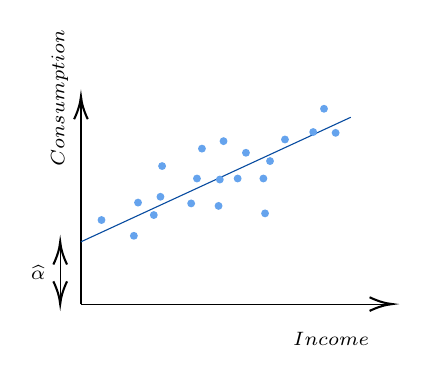
\begin{tikzpicture}[x=0.75pt,y=0.75pt,yscale=-1,xscale=1]
%uncomment if require: \path (0,300); %set diagram left start at 0, and has height of 300

%Straight Lines [id:da7891334212873228] 
\draw    (100,170) -- (100,72) ;
\draw [shift={(100,70)}, rotate = 90] [color={rgb, 255:red, 0; green, 0; blue, 0 }  ][line width=0.75]    (10.93,-3.29) .. controls (6.95,-1.4) and (3.31,-0.3) .. (0,0) .. controls (3.31,0.3) and (6.95,1.4) .. (10.93,3.29)   ;
%Straight Lines [id:da3406060179308057] 
\draw    (100,170) -- (248,170) ;
\draw [shift={(250,170)}, rotate = 180] [color={rgb, 255:red, 0; green, 0; blue, 0 }  ][line width=0.75]    (10.93,-3.29) .. controls (6.95,-1.4) and (3.31,-0.3) .. (0,0) .. controls (3.31,0.3) and (6.95,1.4) .. (10.93,3.29)   ;
%Straight Lines [id:da9291153035165438] 
\draw [color={rgb, 255:red, 6; green, 74; blue, 159 }  ,draw opacity=1 ]   (100,140) -- (230,80) ;
%Shape: Circle [id:dp05271662783949149] 
\draw  [draw opacity=0][fill={rgb, 255:red, 101; green, 163; blue, 237 }  ,fill opacity=1 ] (186.8,126.3) .. controls (186.8,125.25) and (187.65,124.4) .. (188.7,124.4) .. controls (189.75,124.4) and (190.6,125.25) .. (190.6,126.3) .. controls (190.6,127.35) and (189.75,128.2) .. (188.7,128.2) .. controls (187.65,128.2) and (186.8,127.35) .. (186.8,126.3) -- cycle ;
%Shape: Circle [id:dp928567488744433] 
\draw  [draw opacity=0][fill={rgb, 255:red, 101; green, 163; blue, 237 }  ,fill opacity=1 ] (156.4,95.1) .. controls (156.4,94.05) and (157.25,93.2) .. (158.3,93.2) .. controls (159.35,93.2) and (160.2,94.05) .. (160.2,95.1) .. controls (160.2,96.15) and (159.35,97) .. (158.3,97) .. controls (157.25,97) and (156.4,96.15) .. (156.4,95.1) -- cycle ;
%Shape: Circle [id:dp6005536462343878] 
\draw  [draw opacity=0][fill={rgb, 255:red, 101; green, 163; blue, 237 }  ,fill opacity=1 ] (151.2,121.5) .. controls (151.2,120.45) and (152.05,119.6) .. (153.1,119.6) .. controls (154.15,119.6) and (155,120.45) .. (155,121.5) .. controls (155,122.55) and (154.15,123.4) .. (153.1,123.4) .. controls (152.05,123.4) and (151.2,122.55) .. (151.2,121.5) -- cycle ;
%Shape: Circle [id:dp39760046880206923] 
\draw  [draw opacity=0][fill={rgb, 255:red, 101; green, 163; blue, 237 }  ,fill opacity=1 ] (220.8,87.5) .. controls (220.8,86.45) and (221.65,85.6) .. (222.7,85.6) .. controls (223.75,85.6) and (224.6,86.45) .. (224.6,87.5) .. controls (224.6,88.55) and (223.75,89.4) .. (222.7,89.4) .. controls (221.65,89.4) and (220.8,88.55) .. (220.8,87.5) -- cycle ;
%Shape: Circle [id:dp24714164580704323] 
\draw  [draw opacity=0][fill={rgb, 255:red, 101; green, 163; blue, 237 }  ,fill opacity=1 ] (133.2,127.1) .. controls (133.2,126.05) and (134.05,125.2) .. (135.1,125.2) .. controls (136.15,125.2) and (137,126.05) .. (137,127.1) .. controls (137,128.15) and (136.15,129) .. (135.1,129) .. controls (134.05,129) and (133.2,128.15) .. (133.2,127.1) -- cycle ;
%Shape: Circle [id:dp5476889758941296] 
\draw  [draw opacity=0][fill={rgb, 255:red, 101; green, 163; blue, 237 }  ,fill opacity=1 ] (210,87.1) .. controls (210,86.05) and (210.85,85.2) .. (211.9,85.2) .. controls (212.95,85.2) and (213.8,86.05) .. (213.8,87.1) .. controls (213.8,88.15) and (212.95,89) .. (211.9,89) .. controls (210.85,89) and (210,88.15) .. (210,87.1) -- cycle ;
%Shape: Circle [id:dp5389461059835431] 
\draw  [draw opacity=0][fill={rgb, 255:red, 101; green, 163; blue, 237 }  ,fill opacity=1 ] (189.2,101.1) .. controls (189.2,100.05) and (190.05,99.2) .. (191.1,99.2) .. controls (192.15,99.2) and (193,100.05) .. (193,101.1) .. controls (193,102.15) and (192.15,103) .. (191.1,103) .. controls (190.05,103) and (189.2,102.15) .. (189.2,101.1) -- cycle ;
%Shape: Circle [id:dp7999162000916865] 
\draw  [draw opacity=0][fill={rgb, 255:red, 101; green, 163; blue, 237 }  ,fill opacity=1 ] (196.4,90.7) .. controls (196.4,89.65) and (197.25,88.8) .. (198.3,88.8) .. controls (199.35,88.8) and (200.2,89.65) .. (200.2,90.7) .. controls (200.2,91.75) and (199.35,92.6) .. (198.3,92.6) .. controls (197.25,92.6) and (196.4,91.75) .. (196.4,90.7) -- cycle ;
%Shape: Circle [id:dp48490651350831926] 
\draw  [draw opacity=0][fill={rgb, 255:red, 101; green, 163; blue, 237 }  ,fill opacity=1 ] (154,109.5) .. controls (154,108.45) and (154.85,107.6) .. (155.9,107.6) .. controls (156.95,107.6) and (157.8,108.45) .. (157.8,109.5) .. controls (157.8,110.55) and (156.95,111.4) .. (155.9,111.4) .. controls (154.85,111.4) and (154,110.55) .. (154,109.5) -- cycle ;
%Shape: Circle [id:dp0048804619298131735] 
\draw  [draw opacity=0][fill={rgb, 255:red, 101; green, 163; blue, 237 }  ,fill opacity=1 ] (177.6,97.1) .. controls (177.6,96.05) and (178.45,95.2) .. (179.5,95.2) .. controls (180.55,95.2) and (181.4,96.05) .. (181.4,97.1) .. controls (181.4,98.15) and (180.55,99) .. (179.5,99) .. controls (178.45,99) and (177.6,98.15) .. (177.6,97.1) -- cycle ;
%Shape: Circle [id:dp1761655025219515] 
\draw  [draw opacity=0][fill={rgb, 255:red, 101; green, 163; blue, 237 }  ,fill opacity=1 ] (165,110) .. controls (165,108.95) and (165.85,108.1) .. (166.9,108.1) .. controls (167.95,108.1) and (168.8,108.95) .. (168.8,110) .. controls (168.8,111.05) and (167.95,111.9) .. (166.9,111.9) .. controls (165.85,111.9) and (165,111.05) .. (165,110) -- cycle ;
%Shape: Circle [id:dp7464349816264509] 
\draw  [draw opacity=0][fill={rgb, 255:red, 101; green, 163; blue, 237 }  ,fill opacity=1 ] (137.2,103.5) .. controls (137.2,102.45) and (138.05,101.6) .. (139.1,101.6) .. controls (140.15,101.6) and (141,102.45) .. (141,103.5) .. controls (141,104.55) and (140.15,105.4) .. (139.1,105.4) .. controls (138.05,105.4) and (137.2,104.55) .. (137.2,103.5) -- cycle ;
%Shape: Circle [id:dp9536655701011887] 
\draw  [draw opacity=0][fill={rgb, 255:red, 101; green, 163; blue, 237 }  ,fill opacity=1 ] (173.6,109.5) .. controls (173.6,108.45) and (174.45,107.6) .. (175.5,107.6) .. controls (176.55,107.6) and (177.4,108.45) .. (177.4,109.5) .. controls (177.4,110.55) and (176.55,111.4) .. (175.5,111.4) .. controls (174.45,111.4) and (173.6,110.55) .. (173.6,109.5) -- cycle ;
%Shape: Circle [id:dp09880257072760035] 
\draw  [draw opacity=0][fill={rgb, 255:red, 101; green, 163; blue, 237 }  ,fill opacity=1 ] (136.4,118.3) .. controls (136.4,117.25) and (137.25,116.4) .. (138.3,116.4) .. controls (139.35,116.4) and (140.2,117.25) .. (140.2,118.3) .. controls (140.2,119.35) and (139.35,120.2) .. (138.3,120.2) .. controls (137.25,120.2) and (136.4,119.35) .. (136.4,118.3) -- cycle ;
%Shape: Circle [id:dp5038662062572888] 
\draw  [draw opacity=0][fill={rgb, 255:red, 101; green, 163; blue, 237 }  ,fill opacity=1 ] (123.6,137.1) .. controls (123.6,136.05) and (124.45,135.2) .. (125.5,135.2) .. controls (126.55,135.2) and (127.4,136.05) .. (127.4,137.1) .. controls (127.4,138.15) and (126.55,139) .. (125.5,139) .. controls (124.45,139) and (123.6,138.15) .. (123.6,137.1) -- cycle ;
%Shape: Circle [id:dp811482101150289] 
\draw  [draw opacity=0][fill={rgb, 255:red, 101; green, 163; blue, 237 }  ,fill opacity=1 ] (108,129.5) .. controls (108,128.45) and (108.85,127.6) .. (109.9,127.6) .. controls (110.95,127.6) and (111.8,128.45) .. (111.8,129.5) .. controls (111.8,130.55) and (110.95,131.4) .. (109.9,131.4) .. controls (108.85,131.4) and (108,130.55) .. (108,129.5) -- cycle ;
%Shape: Circle [id:dp8603572916171682] 
\draw  [draw opacity=0][fill={rgb, 255:red, 101; green, 163; blue, 237 }  ,fill opacity=1 ] (215.2,75.9) .. controls (215.2,74.85) and (216.05,74) .. (217.1,74) .. controls (218.15,74) and (219,74.85) .. (219,75.9) .. controls (219,76.95) and (218.15,77.8) .. (217.1,77.8) .. controls (216.05,77.8) and (215.2,76.95) .. (215.2,75.9) -- cycle ;
%Shape: Circle [id:dp905215259359926] 
\draw  [draw opacity=0][fill={rgb, 255:red, 101; green, 163; blue, 237 }  ,fill opacity=1 ] (125.6,121.1) .. controls (125.6,120.05) and (126.45,119.2) .. (127.5,119.2) .. controls (128.55,119.2) and (129.4,120.05) .. (129.4,121.1) .. controls (129.4,122.15) and (128.55,123) .. (127.5,123) .. controls (126.45,123) and (125.6,122.15) .. (125.6,121.1) -- cycle ;
%Shape: Circle [id:dp22948995707084874] 
\draw  [draw opacity=0][fill={rgb, 255:red, 101; green, 163; blue, 237 }  ,fill opacity=1 ] (186,109.5) .. controls (186,108.45) and (186.85,107.6) .. (187.9,107.6) .. controls (188.95,107.6) and (189.8,108.45) .. (189.8,109.5) .. controls (189.8,110.55) and (188.95,111.4) .. (187.9,111.4) .. controls (186.85,111.4) and (186,110.55) .. (186,109.5) -- cycle ;
%Shape: Circle [id:dp5690624831381049] 
\draw  [draw opacity=0][fill={rgb, 255:red, 101; green, 163; blue, 237 }  ,fill opacity=1 ] (164.4,122.7) .. controls (164.4,121.65) and (165.25,120.8) .. (166.3,120.8) .. controls (167.35,120.8) and (168.2,121.65) .. (168.2,122.7) .. controls (168.2,123.75) and (167.35,124.6) .. (166.3,124.6) .. controls (165.25,124.6) and (164.4,123.75) .. (164.4,122.7) -- cycle ;
%Shape: Circle [id:dp5707386159913291] 
\draw  [draw opacity=0][fill={rgb, 255:red, 101; green, 163; blue, 237 }  ,fill opacity=1 ] (166.8,91.5) .. controls (166.8,90.45) and (167.65,89.6) .. (168.7,89.6) .. controls (169.75,89.6) and (170.6,90.45) .. (170.6,91.5) .. controls (170.6,92.55) and (169.75,93.4) .. (168.7,93.4) .. controls (167.65,93.4) and (166.8,92.55) .. (166.8,91.5) -- cycle ;
%Straight Lines [id:da9134282789880411] 
\draw    (90,142) -- (90,168) ;
\draw [shift={(90,170)}, rotate = 270] [color={rgb, 255:red, 0; green, 0; blue, 0 }  ][line width=0.75]    (10.93,-3.29) .. controls (6.95,-1.4) and (3.31,-0.3) .. (0,0) .. controls (3.31,0.3) and (6.95,1.4) .. (10.93,3.29)   ;
\draw [shift={(90,140)}, rotate = 90] [color={rgb, 255:red, 0; green, 0; blue, 0 }  ][line width=0.75]    (10.93,-3.29) .. controls (6.95,-1.4) and (3.31,-0.3) .. (0,0) .. controls (3.31,0.3) and (6.95,1.4) .. (10.93,3.29)   ;

% Text Node
\draw (84.4,105.2) node [anchor=north west][inner sep=0.75pt]  [font=\scriptsize,rotate=-270]  {$Consumption$};
% Text Node
\draw (201,182.4) node [anchor=north west][inner sep=0.75pt]  [font=\scriptsize]  {$Income$};
% Text Node
\draw (74.6,150) node [anchor=north west][inner sep=0.75pt]  [font=\scriptsize]  {$\widehat{\alpha }$};


\end{tikzpicture}
\caption{Income vs. Consumption modelled by a linear equation}
\end{marginfigure}

\subsection{Linear models with multiple variables}
We consider the model given by:
\begin{align}
    y=\alpha+\beta_1x_1+\beta_2x_2+\hdots
\end{align}
Such a model is better because:
\begin{enumerate}
    \item We see the effects of other variables on $y$
    \item Fitness of the model improves
\end{enumerate}
For example if $y$ is household consumption and $x_1$ is the income, then $x_i$'s can be other factors like region of stay and number of mouths to feed.

In such models, a new question arises: Which variables do we need to consider. This is decided by two factors:
\begin{enumerate}
    \item \textbf{Economic Theory: }In certain cases we have well established economic theory about the effect of one variable on others. \textbf{Example: }Effects of USD/INR exchange rates on exports.
    \item \textbf{Economic Intuition: }Economists develop an intuition for economic variables and might take decisions based on them.
\end{enumerate}

\subsection{Matrix representation of Linear models}
We define the following matrices:
\begin{align*}
    Y=\begin{bmatrix}y_1\\y_2\\\vdots\\y_n\end{bmatrix}\quad X=\begin{bmatrix}
        1&x_{11}&\hdots&x_{k1}\\
        1&x_{12}&\hdots&x_{k2}\\
        \vdots&\vdots&\ddots&\vdots\\
        1&x_{1n}&\hdots&x_{kn}
    \end{bmatrix}\quad 
    \epsilon=\begin{bmatrix}\epsilon_1\\\epsilon_2\\\vdots\\\epsilon_n\end{bmatrix}\quad
    \beta=\begin{bmatrix}\alpha\\\beta_1\\\beta_2\\\vdots\\\beta_k\end{bmatrix}
\end{align*}
We can represent system of $n$ linear models in $k$ variables in the following way:
\begin{align}
    Y=X\beta+\epsilon
\end{align}
\marginnote{\textbf{For quick reference, the final thing looks like this :} 
$$
\begin{bmatrix}y_1\\y_2\\y_3\\\vdots\\y_n\end{bmatrix}
=\begin{bmatrix}
        1&x_{11}&\hdots&x_{k1}\\
        1&x_{12}&\hdots&x_{k2}\\
        1&x_{13}&\hdots&x_{k3}\\
        \vdots&\vdots&\ddots&\vdots\\
        1&x_{1n}&\hdots&x_{kn}
    \end{bmatrix}\begin{bmatrix}\alpha\\\beta_1\\\beta_2\\\vdots\\\beta_k\end{bmatrix}+\begin{bmatrix}\epsilon_1\\\epsilon_2\\\epsilon_3\\\vdots\\\epsilon_n\end{bmatrix}$$}

Where the $i^{th}$ equation reads:
$$y_i=\alpha+\sum_{r=1}^k x_{r,i}\beta_r+\epsilon_i$$
\subsection{Ordinary Least Squares(OLS) Estimation method}
We want to minimize the errors and one way to do this is by minimizing $\sum_{i=1}^n \epsilon_i^2=\epsilon^t\epsilon$.\sidenote{\textbf{Personal Note: }Things gets tricky here and none of the maths course I have taken has prepared me for this shit. Whatever is written here is found by looking up the following wiki pages: \href{https://en.wikipedia.org/wiki/Residual_sum_of_squares}{RSS},\href{https://en.wikipedia.org/wiki/Total_sum_of_squares}{TSS},\href{https://en.wikipedia.org/wiki/Explained_sum_of_squares}{ESS} and \href{https://en.wikipedia.org/wiki/Ordinary_least_squares}{OLS}. Additionally, explanation of formula is given \href{https://www.youtube.com/watch?v=N7pHym1L9b0&t=380s}{HERE}. Info about matrix calculus can be found \href{https://en.wikipedia.org/wiki/Matrix_calculus}{HERE} and recipes can be found \href{https://www.math.uwaterloo.ca/~hwolkowi/matrixcookbook.pdf}{HERE}.}
\begin{align}
    \epsilon^t\epsilon&=(Y-X\widehat{\beta})^t(Y-X\widehat{\beta})\\
    &=Y^tY-\widehat\beta^tX^tY^t-Y^tX\widehat\beta+\widehat{\beta}^tX^tX\widehat\beta
\end{align}
Now note $M=Y^tX\widehat\beta$ is a scalar. Therefore, $M=M^t$ and $Y^tX\widehat\beta=\widehat\beta^tX^tY^t$. $X^tX$ is a scalar, and we can separate $\widehat{\beta}^tX^tX\widehat\beta$ as $(X^tX)(\widehat\beta^t\widehat\beta)$
Take derivative of 1.8 with respect to $\beta$ to get:

\begin{align}
    \frac{d}{d\beta}\epsilon^t\epsilon=-2X^tY+2X^tX\widehat\beta=0
\end{align}
Simplify to get:
\marginnote{\textbf{List of formulas :}
\begin{align*}
    \frac{\partial x^ta}{\partial x}=\frac{\partial a^tx}{\partial x}=a\\
    \frac{\partial a^tXb}{\partial X}=ab^t\\
    \frac{\partial a^tX^tb}{\partial X}=ba^t\\
    \frac{\partial a^tXa}{\partial X}=\frac{\partial a^tX^ta}{\partial X}=aa^t\\
    \frac{\partial b^tAb}{\partial b}=2Ab=2b^tA
\end{align*}}
\begin{align}
    \widehat\beta=(X^tX)^{-1}X^tY
\end{align}
As long as $X$ is full rank, $X$ is positive and the $\beta$ we obtain is a minimum. We define some terms:
\begin{itemize}
    \item \textbf{Explained sum of squares (ESS)}: A quantity used in describing how well a model, often a regression model, represents the data being modelled. In particular, the explained sum of squares measures how much variation there is in the modelled values.
    \begin{align}
        ESS=\sum_{i=1}^n(\widehat y_i-\bar y)^2
    \end{align}
    \item \textbf{Total sum of squares (TSS or SST)}: A quantity that appears as part of a standard way of presenting results of such analyses. For a set of observations $y_i$, $i \leq n$, it is defined as the sum over all squared differences between the observations and their overall mean.
    \begin{align}
        TSS=\sum_{i=1}^n(y_i-\bar y)^2
    \end{align}
    \item\textbf{Residual sum of squares (RSS)}: The sum of the squares of residuals (deviations predicted from actual empirical values of data). It is a measure of the discrepancy between the data and an estimation model, such as a linear regression. A small RSS indicates a tight fit of the model to the data.
    \begin{align}
        RSS=\sum_{i=1}^n(y_i-\widehat y)^2
    \end{align}
\end{itemize}
We  have the following result:
\begin{align}
    RSS=TSS-ESS
\end{align}
\begin{itemize}
    \item \textbf{Coefficient of determination($R^2$): }It is the proportion of the variation in the dependent variable that is predictable from the independent variable(s).
It is a statistic used in the context of statistical models whose main purpose is either the prediction of future outcomes or the testing of hypotheses, on the basis of other related information. It provides a measure of how well observed outcomes are replicated by the model, based on the proportion of total variation of outcomes explained by the model.\begin{align}
    R^2=\frac{ESS}{TSS}
\end{align}
\marginnote{\textbf{High $R^2$ trap:} Contrary to (my) Expectations, a very high $R^2$ probably means you have messed up your analysis/over-fitted your data. So take care}
\end{itemize}

\section{Non-Linear Models}
Sometimes our data doesn't follow a linear tend. To take care of this we add an additional 
no-linear term to our model. Interpretations of some non-linear models are:
\begin{enumerate}
    \item $y=\alpha+\beta_1\ln x+\epsilon$\\
    It implies a $1\%$ increase in $x$ would increase $y$ by $0.01\beta$ unit.
    \item $\ln y=\alpha+\beta x+\epsilon$\\
    It implies a 1 unit change in $x$ increases $y$ by $\beta$ times.
    \item $\ln y=\alpha+\beta\ln x$\\
    It implies a $1\%$ change in $x$ produces a $\beta\%$ change in $y$ 
\end{enumerate}
An example is given below.
\begin{marginfigure}
    

\tikzset{every picture/.style={line width=0.75pt}} %set default line width to 0.75pt        

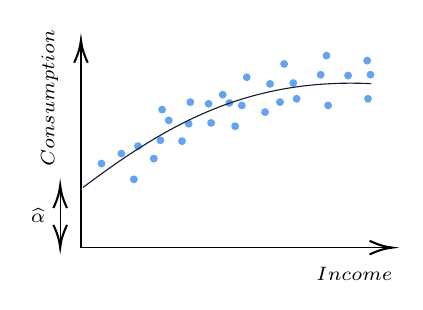
\begin{tikzpicture}[x=0.75pt,y=0.75pt,yscale=-1,xscale=1]
%uncomment if require: \path (0,300); %set diagram left start at 0, and has height of 300

%Straight Lines [id:da7891334212873228] 
\draw    (100,170) -- (100,72) ;
\draw [shift={(100,70)}, rotate = 90] [color={rgb, 255:red, 0; green, 0; blue, 0 }  ][line width=0.75]    (10.93,-3.29) .. controls (6.95,-1.4) and (3.31,-0.3) .. (0,0) .. controls (3.31,0.3) and (6.95,1.4) .. (10.93,3.29)   ;
%Straight Lines [id:da3406060179308057] 
\draw    (100,170) -- (248,170) ;
\draw [shift={(250,170)}, rotate = 180] [color={rgb, 255:red, 0; green, 0; blue, 0 }  ][line width=0.75]    (10.93,-3.29) .. controls (6.95,-1.4) and (3.31,-0.3) .. (0,0) .. controls (3.31,0.3) and (6.95,1.4) .. (10.93,3.29)   ;
%Shape: Circle [id:dp24714164580704323] 
\draw  [draw opacity=0][fill={rgb, 255:red, 101; green, 163; blue, 237 }  ,fill opacity=1 ] (133.2,127.1) .. controls (133.2,126.05) and (134.05,125.2) .. (135.1,125.2) .. controls (136.15,125.2) and (137,126.05) .. (137,127.1) .. controls (137,128.15) and (136.15,129) .. (135.1,129) .. controls (134.05,129) and (133.2,128.15) .. (133.2,127.1) -- cycle ;
%Shape: Circle [id:dp7464349816264509] 
\draw  [draw opacity=0][fill={rgb, 255:red, 101; green, 163; blue, 237 }  ,fill opacity=1 ] (137.2,103.5) .. controls (137.2,102.45) and (138.05,101.6) .. (139.1,101.6) .. controls (140.15,101.6) and (141,102.45) .. (141,103.5) .. controls (141,104.55) and (140.15,105.4) .. (139.1,105.4) .. controls (138.05,105.4) and (137.2,104.55) .. (137.2,103.5) -- cycle ;
%Shape: Circle [id:dp09880257072760035] 
\draw  [draw opacity=0][fill={rgb, 255:red, 101; green, 163; blue, 237 }  ,fill opacity=1 ] (136.4,118.3) .. controls (136.4,117.25) and (137.25,116.4) .. (138.3,116.4) .. controls (139.35,116.4) and (140.2,117.25) .. (140.2,118.3) .. controls (140.2,119.35) and (139.35,120.2) .. (138.3,120.2) .. controls (137.25,120.2) and (136.4,119.35) .. (136.4,118.3) -- cycle ;
%Shape: Circle [id:dp5038662062572888] 
\draw  [draw opacity=0][fill={rgb, 255:red, 101; green, 163; blue, 237 }  ,fill opacity=1 ] (123.6,137.1) .. controls (123.6,136.05) and (124.45,135.2) .. (125.5,135.2) .. controls (126.55,135.2) and (127.4,136.05) .. (127.4,137.1) .. controls (127.4,138.15) and (126.55,139) .. (125.5,139) .. controls (124.45,139) and (123.6,138.15) .. (123.6,137.1) -- cycle ;
%Shape: Circle [id:dp811482101150289] 
\draw  [draw opacity=0][fill={rgb, 255:red, 101; green, 163; blue, 237 }  ,fill opacity=1 ] (108,129.5) .. controls (108,128.45) and (108.85,127.6) .. (109.9,127.6) .. controls (110.95,127.6) and (111.8,128.45) .. (111.8,129.5) .. controls (111.8,130.55) and (110.95,131.4) .. (109.9,131.4) .. controls (108.85,131.4) and (108,130.55) .. (108,129.5) -- cycle ;
%Shape: Circle [id:dp905215259359926] 
\draw  [draw opacity=0][fill={rgb, 255:red, 101; green, 163; blue, 237 }  ,fill opacity=1 ] (125.6,121.1) .. controls (125.6,120.05) and (126.45,119.2) .. (127.5,119.2) .. controls (128.55,119.2) and (129.4,120.05) .. (129.4,121.1) .. controls (129.4,122.15) and (128.55,123) .. (127.5,123) .. controls (126.45,123) and (125.6,122.15) .. (125.6,121.1) -- cycle ;
%Straight Lines [id:da9134282789880411] 
\draw    (90,142) -- (90,168) ;
\draw [shift={(90,170)}, rotate = 270] [color={rgb, 255:red, 0; green, 0; blue, 0 }  ][line width=0.75]    (10.93,-3.29) .. controls (6.95,-1.4) and (3.31,-0.3) .. (0,0) .. controls (3.31,0.3) and (6.95,1.4) .. (10.93,3.29)   ;
\draw [shift={(90,140)}, rotate = 90] [color={rgb, 255:red, 0; green, 0; blue, 0 }  ][line width=0.75]    (10.93,-3.29) .. controls (6.95,-1.4) and (3.31,-0.3) .. (0,0) .. controls (3.31,0.3) and (6.95,1.4) .. (10.93,3.29)   ;
%Shape: Circle [id:dp7365844998297545] 
\draw  [draw opacity=0][fill={rgb, 255:red, 101; green, 163; blue, 237 }  ,fill opacity=1 ] (169.6,100.3) .. controls (169.6,99.25) and (170.45,98.4) .. (171.5,98.4) .. controls (172.55,98.4) and (173.4,99.25) .. (173.4,100.3) .. controls (173.4,101.35) and (172.55,102.2) .. (171.5,102.2) .. controls (170.45,102.2) and (169.6,101.35) .. (169.6,100.3) -- cycle ;
%Shape: Circle [id:dp3788653787421561] 
\draw  [draw opacity=0][fill={rgb, 255:red, 101; green, 163; blue, 237 }  ,fill opacity=1 ] (200.4,90.7) .. controls (200.4,89.65) and (201.25,88.8) .. (202.3,88.8) .. controls (203.35,88.8) and (204.2,89.65) .. (204.2,90.7) .. controls (204.2,91.75) and (203.35,92.6) .. (202.3,92.6) .. controls (201.25,92.6) and (200.4,91.75) .. (200.4,90.7) -- cycle ;
%Shape: Circle [id:dp7089108031522956] 
\draw  [draw opacity=0][fill={rgb, 255:red, 101; green, 163; blue, 237 }  ,fill opacity=1 ] (237.6,86.7) .. controls (237.6,85.65) and (238.45,84.8) .. (239.5,84.8) .. controls (240.55,84.8) and (241.4,85.65) .. (241.4,86.7) .. controls (241.4,87.75) and (240.55,88.6) .. (239.5,88.6) .. controls (238.45,88.6) and (237.6,87.75) .. (237.6,86.7) -- cycle ;
%Shape: Circle [id:dp7585825879013028] 
\draw  [draw opacity=0][fill={rgb, 255:red, 101; green, 163; blue, 237 }  ,fill opacity=1 ] (117.6,124.7) .. controls (117.6,123.65) and (118.45,122.8) .. (119.5,122.8) .. controls (120.55,122.8) and (121.4,123.65) .. (121.4,124.7) .. controls (121.4,125.75) and (120.55,126.6) .. (119.5,126.6) .. controls (118.45,126.6) and (117.6,125.75) .. (117.6,124.7) -- cycle ;
%Shape: Circle [id:dp050137392198690955] 
\draw  [draw opacity=0][fill={rgb, 255:red, 101; green, 163; blue, 237 }  ,fill opacity=1 ] (159.6,100.7) .. controls (159.6,99.65) and (160.45,98.8) .. (161.5,98.8) .. controls (162.55,98.8) and (163.4,99.65) .. (163.4,100.7) .. controls (163.4,101.75) and (162.55,102.6) .. (161.5,102.6) .. controls (160.45,102.6) and (159.6,101.75) .. (159.6,100.7) -- cycle ;
%Shape: Circle [id:dp06868816464921434] 
\draw  [draw opacity=0][fill={rgb, 255:red, 101; green, 163; blue, 237 }  ,fill opacity=1 ] (140.4,108.7) .. controls (140.4,107.65) and (141.25,106.8) .. (142.3,106.8) .. controls (143.35,106.8) and (144.2,107.65) .. (144.2,108.7) .. controls (144.2,109.75) and (143.35,110.6) .. (142.3,110.6) .. controls (141.25,110.6) and (140.4,109.75) .. (140.4,108.7) -- cycle ;
%Shape: Circle [id:dp2888797411517823] 
\draw  [draw opacity=0][fill={rgb, 255:red, 101; green, 163; blue, 237 }  ,fill opacity=1 ] (150,110.3) .. controls (150,109.25) and (150.85,108.4) .. (151.9,108.4) .. controls (152.95,108.4) and (153.8,109.25) .. (153.8,110.3) .. controls (153.8,111.35) and (152.95,112.2) .. (151.9,112.2) .. controls (150.85,112.2) and (150,111.35) .. (150,110.3) -- cycle ;
%Shape: Circle [id:dp053059404218516515] 
\draw  [draw opacity=0][fill={rgb, 255:red, 101; green, 163; blue, 237 }  ,fill opacity=1 ] (236,79.9) .. controls (236,78.85) and (236.85,78) .. (237.9,78) .. controls (238.95,78) and (239.8,78.85) .. (239.8,79.9) .. controls (239.8,80.95) and (238.95,81.8) .. (237.9,81.8) .. controls (236.85,81.8) and (236,80.95) .. (236,79.9) -- cycle ;
%Shape: Circle [id:dp24450380406330308] 
\draw  [draw opacity=0][fill={rgb, 255:red, 101; green, 163; blue, 237 }  ,fill opacity=1 ] (172.4,111.5) .. controls (172.4,110.45) and (173.25,109.6) .. (174.3,109.6) .. controls (175.35,109.6) and (176.2,110.45) .. (176.2,111.5) .. controls (176.2,112.55) and (175.35,113.4) .. (174.3,113.4) .. controls (173.25,113.4) and (172.4,112.55) .. (172.4,111.5) -- cycle ;
%Shape: Circle [id:dp7415319906504264] 
\draw  [draw opacity=0][fill={rgb, 255:red, 101; green, 163; blue, 237 }  ,fill opacity=1 ] (213.6,86.7) .. controls (213.6,85.65) and (214.45,84.8) .. (215.5,84.8) .. controls (216.55,84.8) and (217.4,85.65) .. (217.4,86.7) .. controls (217.4,87.75) and (216.55,88.6) .. (215.5,88.6) .. controls (214.45,88.6) and (213.6,87.75) .. (213.6,86.7) -- cycle ;
%Shape: Circle [id:dp8549550343460292] 
\draw  [draw opacity=0][fill={rgb, 255:red, 101; green, 163; blue, 237 }  ,fill opacity=1 ] (226.8,87.1) .. controls (226.8,86.05) and (227.65,85.2) .. (228.7,85.2) .. controls (229.75,85.2) and (230.6,86.05) .. (230.6,87.1) .. controls (230.6,88.15) and (229.75,89) .. (228.7,89) .. controls (227.65,89) and (226.8,88.15) .. (226.8,87.1) -- cycle ;
%Shape: Circle [id:dp25247407109455566] 
\draw  [draw opacity=0][fill={rgb, 255:red, 101; green, 163; blue, 237 }  ,fill opacity=1 ] (236.4,98.3) .. controls (236.4,97.25) and (237.25,96.4) .. (238.3,96.4) .. controls (239.35,96.4) and (240.2,97.25) .. (240.2,98.3) .. controls (240.2,99.35) and (239.35,100.2) .. (238.3,100.2) .. controls (237.25,100.2) and (236.4,99.35) .. (236.4,98.3) -- cycle ;
%Shape: Circle [id:dp957708644635451] 
\draw  [draw opacity=0][fill={rgb, 255:red, 101; green, 163; blue, 237 }  ,fill opacity=1 ] (166.4,96.3) .. controls (166.4,95.25) and (167.25,94.4) .. (168.3,94.4) .. controls (169.35,94.4) and (170.2,95.25) .. (170.2,96.3) .. controls (170.2,97.35) and (169.35,98.2) .. (168.3,98.2) .. controls (167.25,98.2) and (166.4,97.35) .. (166.4,96.3) -- cycle ;
%Shape: Circle [id:dp9756577608609103] 
\draw  [draw opacity=0][fill={rgb, 255:red, 101; green, 163; blue, 237 }  ,fill opacity=1 ] (186.8,104.7) .. controls (186.8,103.65) and (187.65,102.8) .. (188.7,102.8) .. controls (189.75,102.8) and (190.6,103.65) .. (190.6,104.7) .. controls (190.6,105.75) and (189.75,106.6) .. (188.7,106.6) .. controls (187.65,106.6) and (186.8,105.75) .. (186.8,104.7) -- cycle ;
%Shape: Circle [id:dp6116599141397326] 
\draw  [draw opacity=0][fill={rgb, 255:red, 101; green, 163; blue, 237 }  ,fill opacity=1 ] (202,98.3) .. controls (202,97.25) and (202.85,96.4) .. (203.9,96.4) .. controls (204.95,96.4) and (205.8,97.25) .. (205.8,98.3) .. controls (205.8,99.35) and (204.95,100.2) .. (203.9,100.2) .. controls (202.85,100.2) and (202,99.35) .. (202,98.3) -- cycle ;
%Shape: Circle [id:dp13791923128438754] 
\draw  [draw opacity=0][fill={rgb, 255:red, 101; green, 163; blue, 237 }  ,fill opacity=1 ] (216.4,77.5) .. controls (216.4,76.45) and (217.25,75.6) .. (218.3,75.6) .. controls (219.35,75.6) and (220.2,76.45) .. (220.2,77.5) .. controls (220.2,78.55) and (219.35,79.4) .. (218.3,79.4) .. controls (217.25,79.4) and (216.4,78.55) .. (216.4,77.5) -- cycle ;
%Shape: Circle [id:dp6166488912925998] 
\draw  [draw opacity=0][fill={rgb, 255:red, 101; green, 163; blue, 237 }  ,fill opacity=1 ] (217.2,101.5) .. controls (217.2,100.45) and (218.05,99.6) .. (219.1,99.6) .. controls (220.15,99.6) and (221,100.45) .. (221,101.5) .. controls (221,102.55) and (220.15,103.4) .. (219.1,103.4) .. controls (218.05,103.4) and (217.2,102.55) .. (217.2,101.5) -- cycle ;
%Shape: Circle [id:dp030989830338037372] 
\draw  [draw opacity=0][fill={rgb, 255:red, 101; green, 163; blue, 237 }  ,fill opacity=1 ] (196,81.5) .. controls (196,80.45) and (196.85,79.6) .. (197.9,79.6) .. controls (198.95,79.6) and (199.8,80.45) .. (199.8,81.5) .. controls (199.8,82.55) and (198.95,83.4) .. (197.9,83.4) .. controls (196.85,83.4) and (196,82.55) .. (196,81.5) -- cycle ;
%Shape: Circle [id:dp40384369177751367] 
\draw  [draw opacity=0][fill={rgb, 255:red, 101; green, 163; blue, 237 }  ,fill opacity=1 ] (178,87.9) .. controls (178,86.85) and (178.85,86) .. (179.9,86) .. controls (180.95,86) and (181.8,86.85) .. (181.8,87.9) .. controls (181.8,88.95) and (180.95,89.8) .. (179.9,89.8) .. controls (178.85,89.8) and (178,88.95) .. (178,87.9) -- cycle ;
%Shape: Circle [id:dp44332214446239937] 
\draw  [draw opacity=0][fill={rgb, 255:red, 101; green, 163; blue, 237 }  ,fill opacity=1 ] (175.6,101.5) .. controls (175.6,100.45) and (176.45,99.6) .. (177.5,99.6) .. controls (178.55,99.6) and (179.4,100.45) .. (179.4,101.5) .. controls (179.4,102.55) and (178.55,103.4) .. (177.5,103.4) .. controls (176.45,103.4) and (175.6,102.55) .. (175.6,101.5) -- cycle ;
%Shape: Circle [id:dp9748600936507263] 
\draw  [draw opacity=0][fill={rgb, 255:red, 101; green, 163; blue, 237 }  ,fill opacity=1 ] (189.2,91.1) .. controls (189.2,90.05) and (190.05,89.2) .. (191.1,89.2) .. controls (192.15,89.2) and (193,90.05) .. (193,91.1) .. controls (193,92.15) and (192.15,93) .. (191.1,93) .. controls (190.05,93) and (189.2,92.15) .. (189.2,91.1) -- cycle ;
%Shape: Circle [id:dp4578144194879511] 
\draw  [draw opacity=0][fill={rgb, 255:red, 101; green, 163; blue, 237 }  ,fill opacity=1 ] (160.8,109.9) .. controls (160.8,108.85) and (161.65,108) .. (162.7,108) .. controls (163.75,108) and (164.6,108.85) .. (164.6,109.9) .. controls (164.6,110.95) and (163.75,111.8) .. (162.7,111.8) .. controls (161.65,111.8) and (160.8,110.95) .. (160.8,109.9) -- cycle ;
%Shape: Circle [id:dp7874372208554312] 
\draw  [draw opacity=0][fill={rgb, 255:red, 101; green, 163; blue, 237 }  ,fill opacity=1 ] (150.8,99.9) .. controls (150.8,98.85) and (151.65,98) .. (152.7,98) .. controls (153.75,98) and (154.6,98.85) .. (154.6,99.9) .. controls (154.6,100.95) and (153.75,101.8) .. (152.7,101.8) .. controls (151.65,101.8) and (150.8,100.95) .. (150.8,99.9) -- cycle ;
%Shape: Circle [id:dp7274215207965388] 
\draw  [draw opacity=0][fill={rgb, 255:red, 101; green, 163; blue, 237 }  ,fill opacity=1 ] (146.8,118.7) .. controls (146.8,117.65) and (147.65,116.8) .. (148.7,116.8) .. controls (149.75,116.8) and (150.6,117.65) .. (150.6,118.7) .. controls (150.6,119.75) and (149.75,120.6) .. (148.7,120.6) .. controls (147.65,120.6) and (146.8,119.75) .. (146.8,118.7) -- cycle ;
%Curve Lines [id:da2072090423997458] 
\draw [color={rgb, 255:red, 13; green, 29; blue, 50 }  ,draw opacity=1 ]   (101,141) .. controls (141,111) and (179.8,88.2) .. (239.8,91) ;
%Shape: Circle [id:dp03044071599769671] 
\draw  [draw opacity=0][fill={rgb, 255:red, 101; green, 163; blue, 237 }  ,fill opacity=1 ] (194,99.9) .. controls (194,98.85) and (194.85,98) .. (195.9,98) .. controls (196.95,98) and (197.8,98.85) .. (197.8,99.9) .. controls (197.8,100.95) and (196.95,101.8) .. (195.9,101.8) .. controls (194.85,101.8) and (194,100.95) .. (194,99.9) -- cycle ;

% Text Node
\draw (79.6,132.4) node [anchor=north west][inner sep=0.75pt]  [font=\scriptsize,rotate=-270]  {$Consumption$};
% Text Node
\draw (212.2,178) node [anchor=north west][inner sep=0.75pt]  [font=\scriptsize]  {$Income$};
% Text Node
\draw (74.6,150) node [anchor=north west][inner sep=0.75pt]  [font=\scriptsize]  {$\widehat{\alpha }$};


\end{tikzpicture}
\caption{Non-Linear relation between Income and consumption. Note that the points don't have an exactly linear tendency}
\end{marginfigure}
\begin{tcolorbox}[colback=c4,colframe=c3,title=Example 1.2: Non-Linear modelling consumption with respect to income]
For high income, the linear tendency of fig 1.1 is lost and is more like fig 1.2. To capture the diminishing slope we add a quadratic term to our model. The new model is therefore given by:
\begin{align}
    y=\alpha+\beta_1x+\beta_2x^2+\epsilon
\end{align}
The marginal propensity to consume now is non-constant and is given by $\beta_1+2x\beta_2$. From the fact that the slop is decreasing with income, we conclude $\beta_2$ is negative.
\end{tcolorbox}



















\section{Dealing with categorical parameter}
It might so happen that a parameter we are dealing with is non-continuous and attains a discrete set of values. In that case, Eqn1.6 doesn't apply directly.
\subsection{Parameters that take two values}
We represent discrete parameters by $d$. Our model becomes:
\begin{align}
    y=\alpha+\beta_1x+\beta_2d
\end{align}
Where we assume that calculations are done with respect to a base category. For the category in question we set $d=1$ otherwise(base case) $d=0$. Therefore,
\begin{align}
    E[y|d=0]=\alpha +\beta_1x\quad E[y|d=1]-E[y|d=0]=\beta_2
\end{align}
\begin{tcolorbox}[colback=c4,colframe=c3,title=Example 1.3: Variation of consumption with gender of head of family,breakable]
It is found that consumption habits of household depends on gender of head of household. In female lead households, there is increased consumption of nutritious food. This has prompted governments of Latin American countries to pay cash subsidiaries in the hands of the woman of the house to make sure that the cash is used appropriately.\\
If we consider a male head of the house to be our base case then we have $\beta_2>0$ and if having a woman is the base case we have $\beta_2<0$
\end{tcolorbox}
















\subsection{Parameters that take multiple values}
If a parameter takes $n$ values then we need $n-1$ variables. We fix a base parameter $d_0$. If the $i^{th}$ value is present, we set $d_i=1$ and $d_j(j\ne0)=0$
\begin{align}
    E[y|\text{Parameter takes $i^{th}$ value}]-E[y|\text{Parameter takes base value}]=\beta_i
\end{align}
The whole model reads:
\begin{align}
    y=\alpha+\beta x+\sum_{i=1}^{n-1}\beta_id_i
\end{align}
\marginnote{
\textbf{For quick reference
In case the parameter takes the $i^{th}$ value, the equation reads:}
\begin{align}
    y=\alpha+\beta_i+\beta x
\end{align}
}
\begin{tcolorbox}[colback=c4,colframe=c3,breakable,title=Example 1.4: Variation of income with caste]
In India, one's caste is quite important in deciding one's income. We consider 4 categories:
\begin{enumerate}
    \item \textbf{General:} Considered to be the base case.
    \item \textbf{SC:} Represented by $d_1$
    \item \textbf{ST:} Represented by $d_2$
    \item \textbf{OBC:} Represented by $d_3$
    
\end{enumerate}
Now if $d_1>d_2$ then we can conclude that $SC$ have a higher expected  income than $ST$. Due to the linear nature of Eq1.20, changing which category is taken as base is quite easy. The relevant equations in this case are:
\begin{align*}
    &y=\alpha+\beta x+\beta_1d_1+\beta_2d_2+\beta_3d_3\\
    &y=\alpha+\beta x\quad&\text{For general caste}\\
    &y=\alpha+\beta x+\beta_1\quad&\text{For SC }\\
    &y=\alpha+\beta x+\beta_2\quad&\text{For ST }\\
    &y=\alpha+\beta x+\beta_3\quad&\text{For OBC}
\end{align*}
\end{tcolorbox}
















\section{Confidence in parameters}
\subsection{Estimators}
\textbf{Ref: Casella, Ch7: Point Estimation. \cite{Casella_Berger_20}}\\
Given a data-set we would like to determine the parameters of the relation they are following. But as we are working with a finite dataset we may always get an estimate of a parameter and never the parameter itself. All we claim is the expected value of the estimate is the actual parameter itself. For example consider two variables related by $y=\alpha+\beta x$. We have a dataset given by $\{x_i,y_i\}_{i\in\mathbb{N}}$. We estimate $\widehat\beta$ using some method(like OLS). Then what we claim is $E[\widehat\beta]=\beta$. \\
\textbf{Definition [Point Estimator]: }
A point estimator is a function of the sample.\\
We use an appropriate estimator to estimate the parameters. The definition is purposefully vague to make sure we don't accidentally rule out any candidate. \\
\textbf{Definition [Estimate]: }The realized value of the estimator for some sample is known as the estimate.


\subsection{Variance in estimates}
Due to randomness, it is natural to have some variance in the estimates as a function of the sample. If variance of the estimator is low, then we have a higher confidence in the parameter it is estimating. We make some assumptions here:
\begin{enumerate}
    \item $\epsilon\sim N(0,\sigma^2)$
    \item $\widehat\beta\sim N(\beta,\sigma^2(X^tX)^{-1}$
\end{enumerate}
We define:
$$\text{Standard Error }=\sqrt{\widehat{Var(\widehat\beta)}}=\sqrt{\widehat{\sigma^2(X^tX)}}$$
The estimated error is:
$$\hat{\epsilon}=y-\hat{\alpha}-\hat{\beta}x$$
The estimated variance in estimated error is:
$$\sigma^2=\frac{1}{n-k}\sum\hat{\epsilon_i}^2$$
where 
$$n=\text{Sample Size}$$
$$k=\text{Number of independent in model}$$
The $n-k$ in the denominator is to account for the degrees of freedom so that the estimate is unbiased. For an unbiased estimator of a parameter $p$ we have:
$$E[\hat{p}]=p$$
For a sample size of degree $n$ modelled with $k$ parameters, the degree of freedom is given by $n-k$. We define the $t$ statistic with $n-k$ degree of freedom as $\frac{\hat{\beta}}{S.E(\hat{\beta})}$. If the degrees of freedom is greater than 32, then significance of the $t$-statistic= significance of $\hat{\beta}$ statistic. 
\subsection{Hypothesis testing and measure of significance}
\textbf{Definition [Significance] :}Measure of allowance of error. A significance at $5\%$ level means that the error in the estimation of the parameter is less than $5\%$.\\
At a low level of significance we fail to reject the null hypothesis. This is distinctly different from accepting the alternate hypothesis.


\section{Omitted Variable Bias}
\textbf{Ref: Cameron Trivedi Omitted Variable Bias(Sec 4.7.4) for a more mathematical treatment.\cite{Cameron_Trivedi_2005}}\\\noindent
Suppose $y$ is dependent on $x_1,x_2,x_3$, but we model it based on $x_1,x_2$. This might be done because:
\begin{enumerate}
    \item We lack data on $x_3$
    \item We didn't know that the dependence existed, i.e. there was a mistake.
\end{enumerate}
If $Cov(x_1,x_3)=Cov(x_2,x_3)=0$ then there is no problem in estimates of marginal quantities. The problem arises when this is not the case.

\marginnote{This is a very back of the paper analysis but gives the feel for the thing:
\begin{align*}
    \widehat\beta&=E\left[\frac{\partial y}{\partial x}\right]\\
    &=E\left[\frac{\partial \beta x}{\partial x}+\frac{\partial \beta'x'}{\partial x}+\frac{\epsilon}{\partial x}\right]\\
    &=E\left[\frac{\partial \beta x}{\partial x}\right]+E\left[\frac{\partial \beta'x'}{\partial x}\right]+E\left[\frac{\partial \epsilon}{\partial x}\right]\\
    &=\beta+\beta'E\left[\frac{\partial x'}{\partial x}\right]
\end{align*}
\noindent
Assume $\beta'>0$. Then $\widehat\beta>\beta$ if $Cov(x,x')>0$ and  $\widehat\beta<\beta$ if $Cov(x,x')<0$.
}
For example, let $y=\alpha+\beta x+\beta'x'+\epsilon$ but is modelled as $y=\alpha+\beta x+\epsilon$. Let there be an omitted variable $x'$ such that $Cov(x,x')\ne0$. Then in the modelling the model will capture the effect of $x'$ on $y$ through $x$ and thus the effect of $x$ alone on $y$ is downplayed and the estimate we get will be incorrect.

\begin{tcolorbox}[colback=c4,colframe=c3,title=Example 1.5: Variation of income with age and education]
It is obvious that income increases with both age and education. Suppose one is interested in the effect of education on income (and this interest is important as this is used to formulate the compulsory education plan: we need to have an accurate grasp of how income increases with increase in education, so we know if government funding of education is beneficial). As no. of years of education depends on age, if we don't include the effect of age in our calculations then our estimate of the effect will be biased(\textbf{Ref: Examples of regression in ch3}). By the side-note above we see that the estimate will be higher than the actual value.
\end{tcolorbox}
One naive way to emit omitted variable bias is to consider every variable in the model. But this is not efficient as:
\begin{enumerate}
    \item It is important o simplify the model as much as we can to reduce cost of computation.
    \item Often we don't have enough data. 
\end{enumerate}
\textbf{Ref: Instrumental Variable} for Omitted bias correction. 
\section{Interaction variables}
Suppose there is a categorical variable $d$ which takes two values: 0 and 1. We are interested in knowing variation of the dependent variable $y$ with respect to the independent variable $x$ as $v$ takes different values. We do this by defining an interaction variable $\tilde x=x\times d$(i.e. $\tilde{x_i}=x_id_i$ for all pairs $(x_i,d_i)$ in our dataset). Let our initial model was $y=\alpha+\beta x+\gamma d+\sum_r \beta_r x_r$ where $x_r$'s are the other independent variables in consideration. We define  our new model as $y=\alpha+\beta x+\gamma d+\tilde\beta \tilde{x}+\sum_r \beta_r x_r$. Then we have:
$$\frac{\partial y}{\partial x}=\beta+\tilde\beta d$$
as $\tilde\beta\tilde x=\tilde \beta xd$. Therefore, the marginal change in $y$ with $x$ $\beta$ if $d=0$ and $\beta+\tilde\beta$ if $d=1$.






\chapter{Instrumental Variables}
\section{Introduction}
As mentioned before, direct regression of one variable over other might not give the proper marginal coefficient. In those cases we use instrumental variables.
\section{Endogenity errors}
In econometrics, endogeneity broadly refers to situations in which an explanatory variable is correlated with the error term. Endogenity errors are errors where the independent variable is not uncorrelated with the error terms. Examples of such errors are:
\begin{enumerate}
    \item Omitted variable bias
    \item Measurement errors
\end{enumerate}
There are two ways to correct endogenity errors. They are:
\begin{enumerate}
    \item Using an instrumental variable
    \item Using a structured equation model.
\end{enumerate}
\section{Correction using Instrumental variable}
We look for a variable $z$ which is correlated to the dependent variable but is exogenous to the error term. Such a variable is called an instrumental variable. Such a variable satisfies two main conditions:
\begin{enumerate}
    \item The IV is causally related to $x$(This is generally found by intuition)
    \item The IV is uncorrelated with $\epsilon$(This is verified statistically)
\end{enumerate}

\begin{marginfigure}
    

\tikzset{every picture/.style={line width=0.75pt}} %set default line width to 0.75pt        

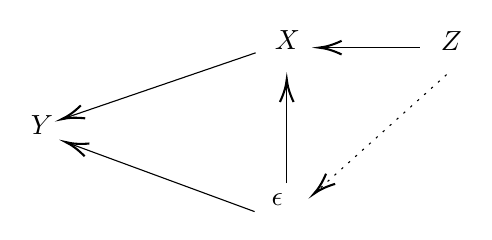
\begin{tikzpicture}[x=0.75pt,y=0.75pt,yscale=-1,xscale=1]
%uncomment if require: \path (0,300); %set diagram left start at 0, and has height of 300

%Straight Lines [id:da7444287109814038] 
\draw    (245,57.25) -- (153.39,88.6) ;
\draw [shift={(151.5,89.25)}, rotate = 341.11] [color={rgb, 255:red, 0; green, 0; blue, 0 }  ][line width=0.75]    (10.93,-3.29) .. controls (6.95,-1.4) and (3.31,-0.3) .. (0,0) .. controls (3.31,0.3) and (6.95,1.4) .. (10.93,3.29)   ;
%Straight Lines [id:da8305785770237464] 
\draw    (244.5,133.75) -- (155.38,100.94) ;
\draw [shift={(153.5,100.25)}, rotate = 20.21] [color={rgb, 255:red, 0; green, 0; blue, 0 }  ][line width=0.75]    (10.93,-3.29) .. controls (6.95,-1.4) and (3.31,-0.3) .. (0,0) .. controls (3.31,0.3) and (6.95,1.4) .. (10.93,3.29)   ;
%Straight Lines [id:da7575118089364972] 
\draw    (260,120) -- (260,72) ;
\draw [shift={(260,70)}, rotate = 90] [color={rgb, 255:red, 0; green, 0; blue, 0 }  ][line width=0.75]    (10.93,-3.29) .. controls (6.95,-1.4) and (3.31,-0.3) .. (0,0) .. controls (3.31,0.3) and (6.95,1.4) .. (10.93,3.29)   ;
%Straight Lines [id:da6707990620756112] 
\draw    (324,54.75) -- (277.5,54.75) ;
\draw [shift={(275.5,54.75)}, rotate = 360] [color={rgb, 255:red, 0; green, 0; blue, 0 }  ][line width=0.75]    (10.93,-3.29) .. controls (6.95,-1.4) and (3.31,-0.3) .. (0,0) .. controls (3.31,0.3) and (6.95,1.4) .. (10.93,3.29)   ;
%Straight Lines [id:da8068887397489296] 
\draw  [dash pattern={on 0.84pt off 2.51pt}]  (337,67.75) -- (274.49,123.91) ;
\draw [shift={(273,125.25)}, rotate = 318.06] [color={rgb, 255:red, 0; green, 0; blue, 0 }  ][line width=0.75]    (10.93,-3.29) .. controls (6.95,-1.4) and (3.31,-0.3) .. (0,0) .. controls (3.31,0.3) and (6.95,1.4) .. (10.93,3.29)   ;

% Text Node
\draw (135.44,86.4) node [anchor=north west][inner sep=0.75pt]    {$Y$};
% Text Node
\draw (253,45.4) node [anchor=north west][inner sep=0.75pt]    {$X$};
% Text Node
\draw (251.5,123.9) node [anchor=north west][inner sep=0.75pt]    {$\epsilon $};
% Text Node
\draw (333,45.9) node [anchor=north west][inner sep=0.75pt]    {$Z$};


\end{tikzpicture}
\caption{The solid line implies correlation. The dashed line implies no correlation.}
\end{marginfigure}

In particular, the new estimate $\hat{\beta}$ is calculated as:
$$\hat\beta_{IV}\equiv \frac{\Delta y/\Delta z}{\Delta x\Delta z}=\frac{(Z^tZ)^{-1}(Z^tY)}{(Z^tZ)^{-1}(Z^tX)}=(Z^tX)^{-1}(Z^tY)$$
We note that this is different from $\hat\beta_{OLS}=(X^tX)^{-1}(X^tY)$
\section{2 step least square(2SLS)}
Given an instrumental variable $x$, this method is used to find $\beta$.
\begin{enumerate}
    \item Regress $z$ on $x$
    \item Predict $\tilde x$ using the above regression
    \item Regress $y$ on $\tilde x$  
\end{enumerate}
Intuitively, this method works because $\tilde x$ is basically $x$ with the effect of $\epsilon$ stripped off (Due to no correlation between $z$ and $\epsilon$, $z$ treats the effect of $\epsilon$ on $x$ as random errors).
\section{Example of 2SLS using simulated data in \faIcon{r-project}}
\subsection{Creation of the simulated dataset}
This requires the $MASS$ package. We simulate $x=0.75+z+v$. We correlate $v$ and $\epsilon$ by $(v,\epsilon)\sim N(0,0,\sum)$ where $\sum$ is the covariance matrix given by $\sum=\begin{bmatrix}
1 &0.8\\
0.8 &1 
\end{bmatrix}$ We therefore have $Cov(x,\epsilon)=Cov(z,\epsilon)$. We model $z\sim N(2,1)$. Set $y=0.25+0.5x+\epsilon$. 
\begin{lstlisting}
    > library("MASS")
    > set.seed(567)
    > n<-10000
    > mu<-c(0,0)
    > cov<-matrix(c(1,0.8,0.8,1),ncol=2)
    > er<-mvrnorm(n,mu,cov)
    > dim(er)
    [1] 10000     2
    > e<-er[ ,1]
    > v<-er[,2]
    > z<-rnorm(n,2,1)
    > x<-0.75+z+v
    > y<-0.25+(0.5*x)+e
\end{lstlisting}
\subsection{2SLS analysis on $x,z,y$}
We shall assume that we only know about $x,y$ and $z$ and do a 2SLS analysis. First we shall do a normal regression of $y$ on $x$ and check the bias. 
\begin{lstlisting}
    > reg<-lm(y~x)
    > summary(reg)
    
    Call:
    lm(formula = y ~ x)
    
    Residuals:
        Min      1Q  Median      3Q     Max 
    -3.3054 -0.5500  0.0093  0.5397  3.5087 
    
    Coefficients:
                 Estimate Std. Error t value Pr(>|t|)    
    (Intercept) -0.855263   0.017967   -47.6   <2e-16 ***
    x            0.895699   0.005799   154.4   <2e-16 ***
    ---
    Signif. codes:  0 "***" 0.001 "**" 0.01 "*" 0.05 "." 0.1 " " 1
    
    Residual standard error: 0.82 on 9998 degrees of freedom
    Multiple R-squared:  0.7047,	Adjusted R-squared:  0.7046 
    F-statistic: 2.385e+04 on 1 and 9998 DF,  p-value: < 2.2e-16
\end{lstlisting} 
As expected, the effect of $x$ is overestimated and there is a positive bias. Now we shall regress $z$ on $x$ and predict $\tilde x=x1$.
\begin{lstlisting}
    > reg1<-lm(x~z)
    > x1<-predict(reg1,data=z)
\end{lstlisting}
Now we shall regress $y$ on $X$ to get $\hat\beta_{IV}$.
\begin{lstlisting}
    > reg2<-lm(y~x1)
    > summary(reg2)
    
    Call:
    lm(formula = y ~ x1)
    
    Residuals:
        Min      1Q  Median      3Q     Max 
    -4.9194 -0.9456  0.0069  0.9678  5.1786 
    
    Coefficients:
                Estimate Std. Error t value Pr(>|t|)    
    (Intercept)  0.23087    0.04166   5.542 3.07e-08 ***
    x1           0.50169    0.01420  35.319  < 2e-16 ***
    ---
    Signif. codes:  0 "***" 0.001 "**" 0.01 "*" 0.05 "." 0.1 " " 1
    
    Residual standard error: 1.423 on 9998 degrees of freedom
    Multiple R-squared:  0.1109,	Adjusted R-squared:  0.1108 
    F-statistic:  1247 on 1 and 9998 DF,  p-value: < 2.2e-16
\end{lstlisting}
We note that $\hat\beta_{IV}$ gives a much better estimate than $\beta_{OLS}$


\chapter{Probit models}
\section{Introduction}
A model which has categorical output can be divided in three types:\
\begin{enumerate}
    \item \textbf{Single choice model: }The dependent variable has two possible outcomes. Examples are: Predicting if a loan/credit card is to be approved, if a student will take a STEM major, etc. Such a variable can be assumed to take two values: 0 or 1
    \item \textbf{Multiple choice model with unordered outcomes: }The dependent variable can have multiple outcomes, but they are unordered. Examples are: Picking one of the multiple streams with equivalent values in college.
    \item \textbf{Multiple choice model with ordered outcomes: }The dependent variable can have multiple outcomes, but they are unordered. One example is  employment status: there are three states: unemployed, part-time employed and full time employed.
\end{enumerate}
Here, we will mainly focus on the models of the first type. If we do an OLS, then there is a possibility that we will get values other than 0 or 1(and in some cases, we might get a negative value as well). So we go for a non-linear model. 
\section{Dummy variables}
A dummy variable is one that takes only the value 0 or 1 to indicate a choice of a single choice model. They can be thought of as numeric stand-ins for qualitative facts in a regression model, sorting data into mutually exclusive categories (such as smoker and non-smoker). We define a cutoff value $c_0$. If $y*$ is the dummy variable corresponding to $y$ and if estimated value of $y*>c_0$ then we assume $y$ takes the value corresponding to $y*=1$ otherwise it takes the values corresponding to $y*=0$. 
\section{Probit model}
Some commonly used models are probit and logit. In particular, $\hat\beta_{probit}=\hat\beta_{logit}\times0.87$. We assume the following:
\begin{enumerate}
    \item $\epsilon\sim N(0,1)$
    \item Parameters $\beta$ and $\sigma^2$ can't be identified separately: one depends on the other. What we instead try to do is identify $\beta/\sigma^2$. In particular, we scale the data so that $\sigma^2=1$
\end{enumerate}
If our model is of the form $y=\alpha+x\beta+\epsilon$ then $y>c\Rightarrow (\alpha-c)+\beta x+\epsilon>0$ Now we can choose $y*$ appropriately to normalize everything to fit our assumption.
\section{Goodness of fit for a probit model}
$R^2$ is no longer a good measure as $y$ takes only two values. A better measurement is the following index:
$$\text{Percent correctly predicted}=\frac{\text{Total no. of correct prediction}}{\text{Total no. of predictions}}$$
If $\hat y$ is the predicted value of $y$ then correct prediction occurs when $(\hat y,y)=(0,0)$ or $(1,1)$. An incorrect prediction occurs when $(\hat y,y)=(0,1)$ or $(1,0)$. We generally assume $c_0=0.5$
\section{Receiver Operating Characteristic(ROC) curve}
This is a plot of $\%$ correct prediction of $y=1$ vs $\%$ incorrect prediction of $y=0$ for varying values of $c_0$. A higher area under the curve implies a better model. For $c=0$ we note that there is no correct prediction of $y=1$ and all prediction of $y=0$ is incorrect. Conversely, for $c=0$ we note that there is no incorrect prediction of $y=1$ and all prediction of $y=0$ is correct.
\section{Use of probit models}
\begin{enumerate}
    \item Used to check if a credit card/loan application is fit. A probit model based on previous customer records is useful in this case.
    \item Used in consulates for application of visa. 
\end{enumerate}
\section{Insample and Outsample Prediction}
Insample Prediction is predicting the result a of the data from the data itself. Outsample prediction is predicting data different from the data used in sample. \% correctly predicted of outsample prediction is a better fitness of test.

















\chapter{Example of data analysis on \faIcon{r-project} using simwagem.txt}
\section{Introduction}
    Here the data is given in text format. Data in this format has two main benefits:
    \begin{enumerate}
        \item It is easier to read
        \item It has a smaller file size
    \end{enumerate}
    The data contains wage analysis of labor market for males. The analysis
    is done separately for males and females because of two reasons:
    \begin{enumerate}
        \item Factors like having a family/kids (social factors) affect wage
        \item There is a pay gap between males and females for the same work. This is discriminatory in nature. 
    \end{enumerate}
    \marginnote{\textbf{Discrimination: }When there is no clear reason for a difference in treatment of one human with respect to other, we say the cause of the difference is discrimination.} 
\section{Preliminary Analysis}

In the preliminary analysis we look at 
\begin{enumerate}
     \item Number of observations
     \item Number of variables
     \item Idea about the parameters and their values
\end{enumerate}
In this case such an analysis may include things like looking at person's id, age, martial status, religion, caste etc. For categorical variables, the majority group is taken as the base. This helps in better presentation.  In $R$ such an analysis can be made with table and summary commands.
\begin{enumerate}
    \item \textbf{Summary: }This is good for continuous data. In our dataset, such variables include age and earning. 
\begin{lstlisting}
 > summary(df$age)
    Min. 1st Qu.  Median    Mean 3rd Qu.    Max. 
   15.00   30.00   38.00   38.36   47.00   60.00 
 > summary(df$earnings)
    Min. 1st Qu.  Median    Mean 3rd Qu.    Max. 
   194.9   431.1   552.4   578.2   697.8  1164.0 
\end{lstlisting}
    \item \textbf{Table: }This is good for discrete data.  In this case, they include things like martial status, religion being muslim, being urban etc. 
\begin{lstlisting}
> table(df$single)
    0     1 
88275 15658 
> table(df$muslim)
    0     1 
89221 14712 
> table(df$urban)
    0     1 
61520 42413 
\end{lstlisting}
\end{enumerate}

We would in general consider years of education to be continuous. But this is not so. We take a look at the following output:
\begin{lstlisting}
> table(df$eduyrs)

    0     5     8    10    12    14    15    18 
26266 13534 20088 16183 10351  2203 11369  3939 
\end{lstlisting}
We note that there are actually only a few values that the column takes. This corresponds to each major step in education: 5 years is primary education,  8 years is middle school, 10 years is matriculation, 12 years is higher secondary education and so on. Note that most people have 10 years of education. Generally, at this stage one is 15 years of age and is able to work legally. Apart from that, there is also government incentives which serves as secondary motivation.

\section{Analysis: Effect of Education on Earning}
We define earning as the money we get for our work. This is different from income and mostly consist of our salary. Income which don't contribute to earning are stuff like money from tenants, interests etc. Take a look at the following code and figure 3.1.
\begin{lstlisting}
> summary(df$earnings)
Min. 1st Qu.  Median    Mean 3rd Qu.    Max. 
194.9   431.1   552.4   578.2   697.8  1164.0 
\end{lstlisting}
\begin{marginfigure}
    \includegraphics[width=\textwidth]{"c3p1.png"}
    \caption{Density plot of monthly earning. It is easy to conclude that people are generally poor.}
\end{marginfigure}
We note the following about employment in India
\begin{enumerate}
    \item The minimum wage is close to the Govt. minimum wage. This is to prevent exploitation.
    \item In rural areas, you are eligible to a job card. The card guarantees 100 days of work per year
    \item In case, the government is unable to procure suitable work for you, then you  still get paid the Govt. mandated minimum wage. 
\end{enumerate}
We do a naive regression of earnings on years of education.
\begin{lstlisting}
    > reg<-lm(earnings~eduyrs,data = df)
    > summary(reg)
    
    Call:
    lm(formula = earnings ~ eduyrs, data = df)
    
    Residuals:
         Min       1Q   Median       3Q      Max 
    -265.999  -79.272    3.259   77.503  275.537 
    
    Coefficients:
                 Estimate Std. Error t value Pr(>|t|)    
    (Intercept) 353.15207    0.54125   652.5   <2e-16 ***
    eduyrs       29.73722    0.05817   511.2   <2e-16 ***
    ---
    Signif. codes:  0 "***" 0.001 "**" 0.01 "*" 0.05 "." 0.1 " " 1
    
    Residual standard error: 101.5 on 103931 degrees of freedom
    Multiple R-squared:  0.7155,	Adjusted R-squared:  0.7155 
    F-statistic: 2.614e+05 on 1 and 103931 DF,  p-value: < 2.2e-16 
\end{lstlisting}
We get  $R^2\sim 71.5\%$. But this analysis is not exactly correct. There are other factors in play. For example, a higher age corresponds to more experience and thus a higher income.
\begin{lstlisting}
    > reg<-lm(earnings~eduyrs+age,data = df)
    > summary(reg)
    
    Call:
    lm(formula = earnings ~ eduyrs + age, data = df)
    
    Residuals:
         Min       1Q   Median       3Q      Max 
    -230.519  -71.704    2.092   74.729  173.149 
    
    Coefficients:
                 Estimate Std. Error t value Pr(>|t|)    
    (Intercept) 135.39391    1.00186   135.1   <2e-16 ***
    eduyrs       30.62081    0.04673   655.3   <2e-16 ***
    age           5.50303    0.02283   241.1   <2e-16 ***
    ---
    Signif. codes:  0 "***" 0.001 "**" 0.01 "*" 0.05 "." 0.1 " " 1
    
    Residual standard error: 81.28 on 103930 degrees of freedom
    Multiple R-squared:  0.8175,	Adjusted R-squared:  0.8175 
    F-statistic: 2.328e+05 on 2 and 103930 DF,  p-value: < 2.2e-16
\end{lstlisting}

We note by also considering age to be an important independent variable controlling education, we have a higher $R^2$ of $\sim 81.7\%$.\sidenote{\textbf{Mincerian Wage Equation: }The Mincerian wage equation models wage by years of schooling and experience in the labour market.(Copied from Wikipedia)}
We now do one more regression  analysis: one which takes all the variable into account. 
\begin{lstlisting}
    > reg<-lm(earnings~age+single+eduyrs+selfemp
    +regularemp+urban+st+sc+obc+muslim+otherr,data=df)
    > summary(reg)
    
    Call:
    lm(formula = earnings ~ age + single + eduyrs + selfemp + regularemp + 
        urban + st + sc + obc + muslim + otherr, data = df)
    
    Residuals:
         Min       1Q   Median       3Q      Max 
    -121.181  -25.954    0.291   33.178  112.668 
    
    Coefficients:
                 Estimate Std. Error t value Pr(>|t|)    
    (Intercept) 101.32540    0.68272 148.415  < 2e-16 ***
    age           5.29716    0.01355 390.972  < 2e-16 ***
    single       -3.19974    0.41293  -7.749 9.36e-15 ***
    eduyrs       26.38504    0.02648 996.250  < 2e-16 ***
    selfemp      23.90837    0.33478  71.415  < 2e-16 ***
    regularemp   45.48712    0.38584 117.892  < 2e-16 ***
    urban       138.32079    0.26696 518.132  < 2e-16 ***
    st           -7.68017    0.45671 -16.816  < 2e-16 ***
    sc           -9.20168    0.40521 -22.708  < 2e-16 ***
    obc          -7.04464    0.30392 -23.179  < 2e-16 ***
    muslim       -7.45145    0.37556 -19.841  < 2e-16 ***
    otherr       -3.00097    0.45105  -6.653 2.88e-11 ***
    ---
    Signif. codes:  0 "***" 0.001 "**" 0.01 "*" 0.05 "." 0.1 " " 1
    
    Residual standard error: 40.06 on 103921 degrees of freedom
    Multiple R-squared:  0.9557,	Adjusted R-squared:  0.9557 
    F-statistic: 2.037e+05 on 11 and 103921 DF,  p-value: < 2.2e-16
\end{lstlisting}
We note that taking more variables improves our estimates $R^2$. This regression is important because of the following fact: of all the factors that contribute to education, no. of years of education is the only variable that can be improved by government policy. In particular, we note one year of education improved income by $\rupee 26.39$. This analysis is also done with $log$ i.e how many times does the earnings increase with education(\textbf{Ref: Non-Linear models}). 
\begin{lstlisting}
    > df$lnearnings<-log(df$earnings)
    > reg<-lm(lnearnings~age+single+eduyrs+selfemp
    +regularemp+urban+st+sc+obc+muslim+otherr,data=df)
    > summary(reg)
    
    Call:
    lm(formula = lnearnings ~ age + single + eduyrs + selfemp + regularemp + 
        urban + st + sc + obc + muslim + otherr, data = df)
    
    Residuals:
         Min       1Q   Median       3Q      Max 
    -0.43261 -0.02919  0.01062  0.04444  0.16697 
    
    Coefficients:
                  Estimate Std. Error  t value Pr(>|t|)    
    (Intercept)  5.433e+00  1.125e-03 4829.045  < 2e-16 ***
    age          9.741e-03  2.233e-05  436.292  < 2e-16 ***
    single      -5.662e-03  6.805e-04   -8.320  < 2e-16 ***
    eduyrs       4.741e-02  4.364e-05 1086.157  < 2e-16 ***
    selfemp      7.126e-02  5.517e-04  129.162  < 2e-16 ***
    regularemp   9.372e-02  6.358e-04  147.396  < 2e-16 ***
    urban        2.088e-01  4.399e-04  474.592  < 2e-16 ***
    st          -1.375e-02  7.526e-04  -18.272  < 2e-16 ***
    sc          -8.478e-03  6.678e-04  -12.696  < 2e-16 ***
    obc         -2.349e-03  5.008e-04   -4.690 2.74e-06 ***
    muslim      -8.332e-03  6.189e-04  -13.462  < 2e-16 ***
    otherr       1.585e-03  7.433e-04    2.132    0.033 *  
    ---
    Signif. codes:  0 "***" 0.001 "**" 0.01 "*" 0.05 "." 0.1 " " 1
    
    Residual standard error: 0.06601 on 103921 degrees of freedom
    Multiple R-squared:  0.9606,	Adjusted R-squared:  0.9606 
    F-statistic: 2.305e+05 on 11 and 103921 DF,  p-value: < 2.2e-16
\end{lstlisting}
Therefore, 1 year of education increases income by $4.7 \%$
\marginnote{We note that being single decreases income. This is because, generally, being married implies that you have enough income to support your family}

\section{Analysis: Is return to education higher in urban area?}
\textbf{Ref: Interaction Variables}\\
This is a direct application of interaction variables. We show the required code and output below. 
\begin{lstlisting}
    > df$interact<-df$eduyrs*df$urban
    > reg<-lm(earnings~age+single+eduyrs
    +selfemp+regularemp+urban+st+sc+obc+muslim+otherr+interact,data=df)
    > summary(reg)
    
    Call:
    lm(formula = earnings ~ age + single + eduyrs + selfemp + regularemp + 
        urban + st + sc + obc + muslim + otherr + interact, data = df)
    
    Residuals:
        Min      1Q  Median      3Q     Max 
    -45.744  -6.806  -0.004   6.808  50.282 
    
    Coefficients:
                  Estimate Std. Error  t value Pr(>|t|)    
    (Intercept) 148.831707   0.176647  842.536  < 2e-16 ***
    age           5.000869   0.003430 1458.019  < 2e-16 ***
    single       -3.196287   0.104279  -30.651  < 2e-16 ***
    eduyrs       20.058044   0.008424 2380.935  < 2e-16 ***
    selfemp      27.115272   0.084584  320.574  < 2e-16 ***
    regularemp   48.728864   0.097472  499.926  < 2e-16 ***
    urban        18.452035   0.118166  156.154  < 2e-16 ***
    st           -8.126321   0.115336  -70.458  < 2e-16 ***
    sc           -5.025905   0.102386  -49.088  < 2e-16 ***
    obc          -3.021164   0.076819  -39.328  < 2e-16 ***
    muslim       -0.668853   0.095001   -7.040 1.93e-12 ***
    otherr       -0.485820   0.113924   -4.264 2.01e-05 ***
    interact     14.952930   0.012106 1235.158  < 2e-16 ***
    ---
    Signif. codes:  0 "***" 0.001 "**" 0.01 "*" 0.05 "." 0.1 " " 1
    
    Residual standard error: 10.12 on 103920 degrees of freedom
    Multiple R-squared:  0.9972,	Adjusted R-squared:  0.9972 
    F-statistic: 3.055e+06 on 12 and 103920 DF,  p-value: < 2.2e-16
\end{lstlisting}
Therefore, in urban areas, one year of education gives an additional income of $\rupee 14.95$

\section{Prediction: Being self-employed}
In most first world countries, being self-employed is a sign of entrepreneur mindset i.e. someone who has big ideas and is willing to work towards it. On the other hand, in Third World countries, this is often an indentation that a person has failed to secure a stable job. In our data set, if a person is self-employed, it is marked as 0. We try to model it based on age, education, location(urban or rural) and martial status. 
\begin{lstlisting}
    > probit1<-glm(selfemp~age+eduyrs+urban+single,
    family=binomial(link="probit"),data=df)
    > summary(probit1)
    
    Call:
    glm(formula = selfemp ~ age + eduyrs + urban + single, family = binomial(link = "probit"), 
        data = df)
    
    Deviance Residuals: 
        Min       1Q   Median       3Q      Max  
    -1.5117  -1.1062  -0.6935   1.1619   1.9103  
    
    Coefficients:
                  Estimate Std. Error z value Pr(>|z|)    
    (Intercept) -0.5237845  0.0189361  -27.66   <2e-16 ***
    age          0.0165732  0.0004227   39.20   <2e-16 ***
    eduyrs      -0.0099715  0.0007519  -13.26   <2e-16 ***
    urban       -0.2425356  0.0082958  -29.24   <2e-16 ***
    single      -0.3917176  0.0136754  -28.64   <2e-16 ***
    ---
    Signif. codes:  0 "***" 0.001 "**" 0.01 "*" 0.05 "." 0.1 " " 1
    
    (Dispersion parameter for binomial family taken to be 1)
    
        Null deviance: 143251  on 103932  degrees of freedom
    Residual deviance: 136823  on 103928  degrees of freedom
    AIC: 136833
    
    Number of Fisher Scoring iterations: 4
    
    > pr<-predict(probit1,type="response",data=df)
    > yhat<-as.numeric(pr>0.5)
\end{lstlisting}
Now once we have the predicted values of $y$(which is yhat) we can find $\%$ correctly  predicted.
\begin{lstlisting}
    > c_pr<-as.numeric(df$selfemp==yhat)
    > table(c_pr)
    c_pr
        0     1 
    41855 62078 
\end{lstlisting}
The index can be easily calculated after this. 
\section{Analysis: Fitness of probit model}
\textbf{Ref: Insample vs. Outsample prediction}\\
We first divide the data in two parts: one for training and one for testing
\begin{lstlisting}
    > nrow(df)
    [1] 103933
    > df$n<-seq(1,nrow(df),1)
    > train<-df[df$n<51966,]
    > test<-df[df$n>51966,]
\end{lstlisting}
Now we model the train data and test it on test data.
\begin{lstlisting}
    > probit<-glm(selfemp~age+eduyrs+urban+single,family=binomial(link="probit"),data=train)
    > pr<-predict(probit1,type="response",newdata=test)
    > yhat<-as.numeric(pr>0.5)
    > c_pr<-as.numeric(test$selfemp==yhat)
    > x<-table(c_pr)
    > x
    c_pr
        0     1 
    21308 30659 
    > x[2]/(x[1]+x[2])
            1 
    0.5899706 
\end{lstlisting}
The \% correctly predicted in outsample prediction is $\approx$ 59\%















\chapter{\faIcon{r-project} cookbook}
\textit{Note: Due to randomness, there might be small deviations from the data shown here. This is OK}
\section{Introduction to \faIcon{r-project} environment}
\begin{enumerate}
    \item To get current working directory
    \begin{lstlisting}
> getwd()
[1] "/MS/ag19ms129"
    \end{lstlisting}
    \item To change working directory
    \begin{lstlisting}
> setwd("~/Documents/HU codes")
> getwd()
[1] "/MS/ag19ms129/Documents/HU codes"
    \end{lstlisting}
    \item Simulate a normal distribution of $x$ with 
$n=10000,\mu=50,\sigma=5$ and $e$ with $n=10000,\mu=0,\sigma=5$
\begin{lstlisting}
> x<-rnorm(10000,50,5)
> e<-rnorm(10000,0,5)
\end{lstlisting}
Here $\shortleftarrow$ is the assignment operator. $rnorm(n,\mu,\sigma)$ generates a $n$ large dataset with mean $\mu$ and variance $\sigma$. Thus, the first line means the variable is assigned the value $x$
\item Check mean of $x$, variance of $x$ and how distribution of $e$ looks like
\begin{marginfigure}
\includegraphics[width=\textwidth]{"c2s1p1.png"}
\caption{Density plot of $e$. The main thing to note is the rough bell shaped figure}
\end{marginfigure}
\begin{lstlisting}
> mean(x)
[1] 49.88043
> var(x)
[1] 24.90584
> de<-density(e)
> plot(de)
\end{lstlisting}
\item Simulate $y=2.5+0.75x+e$
\begin{lstlisting}
> y<-2.5+(0.75*x)+e
> mean(y)
[1] 39.94653
> var(y)
[1] 39.66292
\end{lstlisting}
\item Make required $X$ matrix
\begin{marginfigure}
    \centering
    \includegraphics[width=0.6\textwidth]{"c2s1p2.png"}
    \caption{How $X$ looks like. Snippet from $R-Studio$}
\end{marginfigure}
\begin{lstlisting}
> X<-matrix(data=NA,10000,2)
> X[,1]<-1
> X[,2]<-x
\end{lstlisting}
Leaving the first entry blank implies change is to be applied to all the columns
\item We now make the required  $Y$ matrix. We do like we did for $X$
\begin{lstlisting}
> Y<-matrix(data=NA,10000,1)
> Y[,1]<-y
\end{lstlisting}
\end{enumerate}
\section{Analysis}
Once we have a simulated $X$ and $Y$, we shall pretend to not know about the relation between them, and try to find estimates parameters $\alpha$ and $\beta$ (as per eqn1.1) which might have generated this.\\\noindent There are commands to automate most of the things needed. But we will work through all the steps once to get a feel for things.
\subsection{Manual Walk-through}
\begin{enumerate}
    \setcounter{enumi}{7}
    \item We will find $\widehat\beta$ using eqn1.11 First we shall calculate $(X^tX)^{-1}$ and call it $XtXi$. Then we shall calculate $X^tY$ and call it $XtY$. Then we multiply them to get $B$ (our estimate of $\widehat\beta$). This, of course, can be done in a single step. Note that the $solve(M)$ command is used to find inverse of matrix $M$. To get product of two matrices $A,B$ we use $A\%*\%B$\sidenote{\textbf{Inaccurate $\widehat\alpha$ fix:}\\\noindent
One might notice that their $\widehat\alpha$ is rather inaccurate. This is OK: the most important thing is accuracy of $\widehat\beta$}
    \begin{lstlisting}
> XtXi<-solve(t(X)%*%X)
> XtY<-t(X)%*%Y
> B<-(XtXi)%*%XtY
> B
          [,1]
[1,] 2.0679723
[2,] 0.7593873
    \end{lstlisting}
Therefore, we get:
\begin{align}
    \widehat\alpha=2.06\hdots\quad\widehat\beta=0.759\hdots
\end{align}
\item{Finding the standard error manually}

\subsection{Analysis of simwagem}

    
\end{enumerate}







\backmatter

\bibliography{sample-handout}
\bibliographystyle{plainnat}


\printindex

\end{document}

